\chapter{Suggested method for importing FKB into OpenStreetMap}
Proof of concept 

\section{Micro-tasking method?}
% Går tilbake til metodene, hva kan vi lære i Norge hvor vi ikke har Mapbox. Norske FKB er bedre enn de man har importert i andre land
% Er dette beste metode?
%Hvordan dele opp i tasking områder? telle antall hus. 50-30-20 hus innenfor hver task? Dette er en utfordring, men er utenfor scopet til oppgaven. Komme med noen tanker rundt hvordan det kan løses. 
Chapter \ref{ch:importmethods} introduce three common import methods, one of them is the micro-tasking method. The micro-tasking method stand out as the best alternative when considering the three methods. Especially together with a micro-tasking tool like the OSM Tasking Manager. The method and tool together solve problems other import methods face. When using them it is not necessary to create a personal dev-website with a list of an import queue like Dave Hansen did during the Tiger import \ref{Hansen2007a} or creating a personal drive folder with the import files, like the OSM user tibnor did during N50 import. The micro-tasking method with the correct tool simplifies the import process.  

The micro-tasking method is of course dependent on a good tool that organize the tasks well. The tasks should be easy to select, to download, to comment on and to mark as resolved. Information about the import and how to complete the tasks should be available and easy to understand. 

The first challenge when using the micro-tasking method is dividing the dataset into smaller parts which give manageable sized tasks. Dividing the building datasets was a challenge in both the New York- and Los Angeles building import, introduced in section \ref{sec:importmicro}. Both solved this issue by dividing it into smaller parts using already defined subregions.*%Gir denne setningen mening?
 When considering the FKB building datasets, instead of dividing it into predefined regions, another alternative is to create subregions by counting buildings. The density of buildings varies between different areas in Norway. %The building density differs between city centers in the municipalities, and between regions outside the city center. 
 The counting approach would ensure that every task has a manageable size. The number of buildings within each task could be from 20-30 units. This number must off course be tested with a test import before a final decision is made. What's important is that finishing a task should not take more than a few hours maximum, but at the same time should not be too small either. Too small tasks can result in too many tasks. *%And? finish the sentence
  
A huge advantage in both New York and Los Angeles import was Mapbox. Having a company involved with professional staff who gets paid is challenging to replace. Luckily the tools created during both imports is open source, available at github. Before implementing any new tool, the FKB building import team should look at already created tools.  

\section{FKB to OSM tagging}
%Hvilke tagger skal brukes for hva
%Skal vi bruke relations med 3D støtte? 

An example of a area representation of a building feature type is shown in listing \ref{eq:buildingfootpr}. This can be used as the building footprint when converting FKB to OSM. This will create the 2D modeling. 

\lstset{
    language=XML,
    morekeywords={encoding,node, tag},
    label=eq:buildingfootpr,
    caption=Example of a area representation of a building feature type in SOSI. 
}
\begin{lstlisting}
.FLATE 715235:
..OBJTYPE Bygning
..KOMM 1601
..BYGGNR 182720836
..BYGGTYP_NBR 111
..BYGGSTAT TB
..KOPIDATA
...OMRÅDEID 1601
...ORIGINALDATAVERT "Trondheim kommune"
...KOPIDATO 20160502
..REF :166806
..NØ
703610900 55898600
\end{lstlisting}

Using figure \ref{fig:buildtypTrd} of the twenty most common building types in Trondheim, there are in total about 140 different types \cite{SOSI-sekretariatet}. Not all building types used in FKB can directly translate to OSM. In the taginfo web page users can search for values commonly used on the building key. The taginfo page was helpful when transferring the FKB building types over to building values in OSM. For instance, type 181 is garage, 111 is detached house (\textit{enebolig}) and 121 is house and are the three most common building types in Trondheim. A list of the 40 most common building types transferred into building values in OSM is in the appendix, table \ref{tab:fkbtoosmdel1} and \ref{tab:fkbtoosmdel1}. 

\begin{figure}[H]
    \centering
    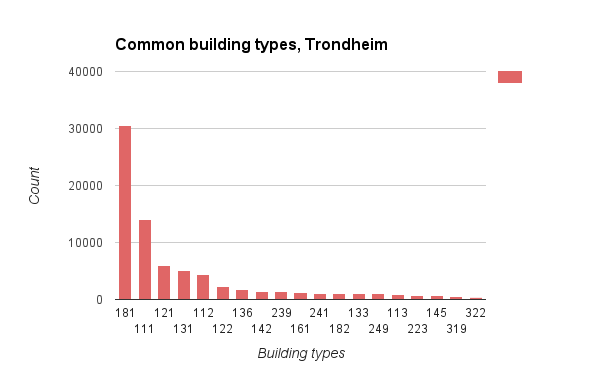
\includegraphics[scale=0.5]{figures/FixedByMe/buildtypestrd.png}
    \caption{20 most common building types in Trondheim, source: postgis query in the cadastre} 
    \label{fig:buildtypTrd}
\end{figure}

These values will represent the value for the building key given to the building feature type. The building feature in listing \ref{eq:buildingfootpr} will be given the value detached (building=detached).  


\section{Conversion using existing script}\label{sec:sosi2osm}
% fkbbuilding.lua
%Lage utkast til en luafil, vise hvordan xml oppsettet blir 

The sosi2osm script was developed in 2013 by the github user Gnonthgol. It was created during the N50 imports initial stages.*%Finn kilden   
 The script is open source and the repository is available at Gnonthgol's GitHub account. The sosi2osm repository do not have any documentation, the only available help is a wiki page who shortly explain how to install and run the code. It is very difficult to install, especially if you don't have a linux operating system. 
 
The script depends on fyba. An open source code distributed by the National Mapping Authority of Norway (Kartverket) to read and write SOSI files. Sosi2osm do not support SOSI files encoded in UTF-8. This is a challenge since FKB sosi files can be UTF-8 encoded.*%Er FKB alltid UTF8 eller bare i noen kommuner?
 This is a major drawback with this script. To test the script, after managing to install it correctly, the first step is to encode the FKB SOSI file into ISO8859-10. This step should not have been necessary.  %Er alle SOSI filer i UTF 8 idag?

When running the script, input is a sosi file and a lua script. A new lua script needs to be created for every conversion desired. In the N50 import they created a lua file for land cover (\textit{arealdekke}), there is also a lua file for address import. The lua file creates key-value pairs from the metadata of the input file. Important metadata in sosi files is the feature type (\textit{OBJTYPE}). In FKB building another important attribute is $BYGGTYP\_NBR$ which give information of what kind of building it is. 

To test the sosi2osm script on the FKB building dataset a fkbbuilding.lua file was created. Using only the most common feature type in the dataset shown in figure \ref{fig:commfeattypes}*.%Ref tabell
  Adding values to the building key, which depend on the buildingtype code from FKB, I used table \ref{tab:fkbtoosmdel1} and \ref{tab:fkbtoosmdel1}. See listing \ref{eq:luabuldtype} for the code snip checking the building value. This code snip checks the $BYGGTYP\_NBR$ attribute value to determine the buildings particular usage. The building=* key-value pair will be placed on the buildings footprint, since only building feature in FKB has this attribute value. 

It is not possible to add height in ways and node representations. Another problem with the sosi2osm script is that it do not consider height values, creating one node for each north, east coordinate pair. If two crossing building lines have different height values they should not share the same node \cite{OpenStreetMap2015}. This is a problem, especially when considering 3D modeling of buildings. 


\section{How to map FKB buildings in 3D}
%Her kan jeg lage et eksempel på hvordan 3D bygg kan moduleres i OSM XML format. 
In order to create a XML representation capable of modeling FKB buildings in 3D, a standard approach should be developed. Members of the OpenStreetMap community, with interest in 3D mapping, started in March 2012 to unite all the separated approaches to model 3D buildings using OSM XML \cite{OpenStreetMapm}. They arranged workshops, which resulted in a suggestion for a simple 3D building schema. This is the approach mentioned in section \ref{buildOSM}. This approach is fairly easy to implement, if the building's roof shape is known. This is not the case for the FKB buildings, so the simple 3D building schema needs modification. Buildings in FKB is modelled with ridge and edge lines and they can be used to create 3D models, see the figures in section \ref{sec:FKBbuilding}. When using ridge and edge modeling, roof shape tags are ignored, meaning the shape of the roof is not needed. Collecting ridge- and edge-lines for one building, creating a way-representation for each line with roof:edge and roof:ridge key's on each. The way-tag representing the building outline, most often the roof-edge feature, holds the height and roof:height information.*%Funker ikke paa alle type bygninger, bare de som har en closed-way rundt hele omrisset
 The listing shown in \ref{eq:3D_fkbbuilding} creates a 3D representation of a house in OSM from FKB data. The house is shown in figure \ref{fig:3DFKBbuild}, using the JOSM editor to generate the code in listing \ref{eq:3D_fkbbuilding} and getting 3D visualization using the JSOM plugin kendzi3d. 

\begin{figure}[H]
    \centering
    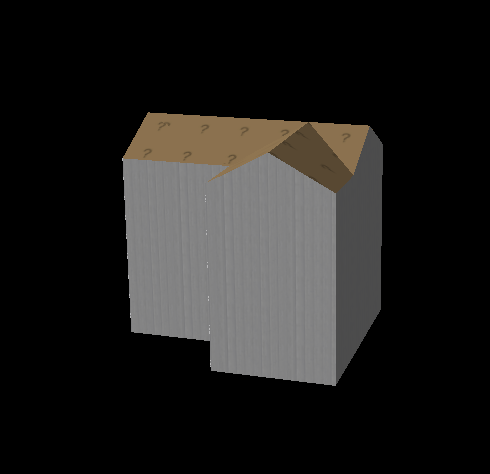
\includegraphics[scale=0.5]{figures/FixedByMe/3DFKBbuilding.png}
    \caption{3D representation of a FKB building, result of listing \ref{eq:3D_fkbbuilding}}
    \label{fig:3DFKBbuild}
\end{figure}

In OpenStreetMap, building height is the distance between the lowest possible position with ground contact and the top of the roof of the building, excluding antennas, etc \cite{OSMwikipage2016}. Height of buildings in FKB is height above sea level. This is a new challenge when mapping FKB buildings in OSM. In listing \ref{eq:3D_fkbbuilding} height above sea level is manually withdrawn from the height given from the FKB data. 

The problem with not distinguishing between overlapping nodes with different heights, mentioned in section \ref{sec:sosi2osm}, make 3D modeling of buildings with overlapping roof ridges and edges a challenge. This problem is shown in figure \ref{fig:3DFKBbuildFail}. Here it's easy to see the effect of overlapping points, they should be located in different heights, but share nodes when using the sosi2osm script.  

\begin{figure}[H]
    \centering
    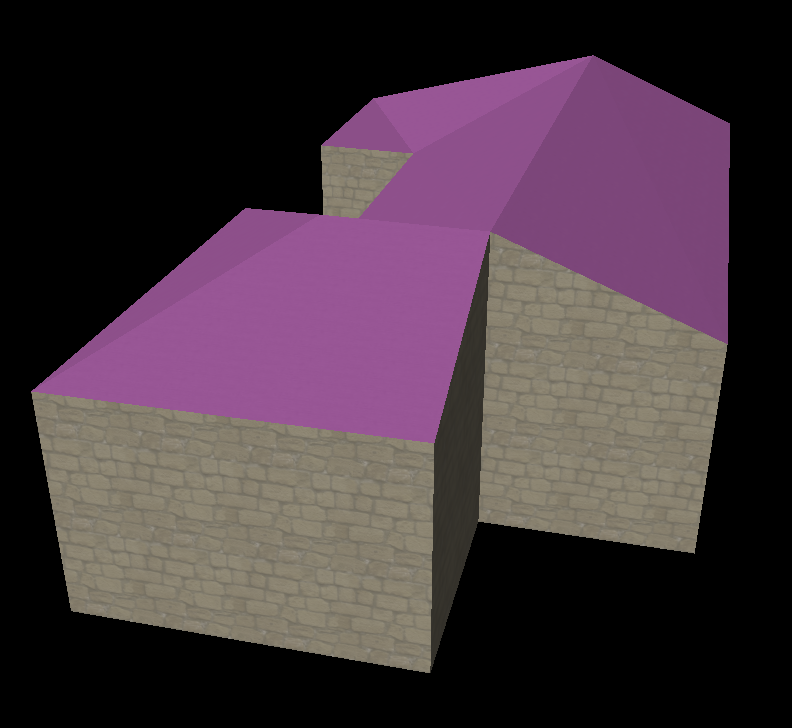
\includegraphics[scale=0.7]{figures/FixedByMe/samenode_but_have_diff_height.png}
    \caption{3D representation of a FKB building}
    \label{fig:3DFKBbuildFail}
\end{figure}

There are different tools developed to visualizing 3D buildings with data from OSM. A problem is that not all tools supports the different modelling. A list of which of them who supports the simple 3D building schema is located at the OSM simple 3D buildings wiki page, most tools accept this schema. 7 tools supports building:part=yes %http://wiki.openstreetmap.org/wiki/3D_Development/Tagging#Usage_Community
2D renderers ignore building:part=* tags, only displaying the building outline. %kanskje vise hvordan huset ser ut i demo.f4map.com?

\section{Evaluation}
From the beginning of the New York building import a goal was to help the city government maintain its building and address datasets \cite{Barth2014b}.  An edit in OSM can be a signal that the building has changed or the imported data is wrong. To help, the New York GIS department subscribes to daily email notifications to building and address changes in OSM. A very good example of how government and open source *%Riktig m open source her?
  can take advantage of each other. 